\documentclass{article}
\usepackage{graphicx}

\begin{document}

\author{Andrew Bartnof,for RMI}
\title{Difference-in-Difference Study for GGRF}
\date{\today}
\maketitle

\section{Introduction}

This paper documents my difference-in-difference (\emph{DiD}) analyses for the GGRF insurance project, in which I attempt to quantify the impact of a green energy project on a neighborhood's home appreciation rates.
I present a mixed-effects model in the main part of this paper.
In the appendix, I present an alternative model, which uses a more conventional two-way fixed-effect DiD schema, but is probably less useful.

\section{Brief Background}

If green energy projects (eg solar farms and wind turbines) are built near residential areas, these projects could impact local home values.
If these homes near green energy projects either appreciate slower, or depreciate faster, than other homes which are not near green energy projects, then home-owners are incentivized to adopt a NIMBY stance, and resist green projects in their neighborhoods-- even if they support green projects in general.

We want to quantify the rate in which which homes appreciate near green energy projects and compare it to baseline home appreciation rates, so that we can help to develop a new kind of financial project; a parametric risk insurance payout for home-owners near green energy projects.
The idea is that, for a limited amount of time, while the green energy projects might artificially depress local homes' values, any home-owner that sells their house could be compensated for this drop in home-value.


\section{Data}

I use four readily-available datasets in this analysis:

\subsection{Zillow Home Prices}
The Zillow home price dataset\footnote{ZHVI All Homes (SFR, Condo/Co-op) Time Series, Smoothed, Seasonally Adjusted. https://www.zillow.com/research/data/} lists the home prices for 26,344 zip-codes, between the years 2000 and 2024.

\subsection{Large-Scale Solar Photovoltaic Sites}
The solar dataset\footnote{Fujita, K.S., Ancona, Z.H., Kramer, L.A. et al. Georectified polygon database of ground-mounted large-scale solar photovoltaic sites in the United States. Sci Data 10, 760 (2023). https://doi.org/10.1038/s41597-023-02644-8} lists the locations and years of operation of thousands of large-scale solar photovoltaic sites.
Note that Ben Hoen is an author of both this dataset and the turbine dataset.

\subsection{Wind Turbines}
This dataset\footnote{
Rand, J.T., Kramer, L.A., Garrity, C.P. et al. A continuously updated, geospatially rectified database of utility-scale wind turbines in the United States. Sci Data 7, 15 (2020). https://doi.org/10.1038/s41597-020-0353-6} lists the locations and years of operation of thousands of wind turbines.

\subsection{Zip-Codes Shape Files}
The zip-code shape file\footnote{https://www.census.gov/programs-surveys/geography/guidance/geo-areas/zctas.html} is the Census program's representation of each zip-code in the nation, circa 2020.
The zip-code dataset is used as a linking document only.


\subsection{Data Notes}

Each observation in the solar and turbine datasets is represented as a polygon, drawn upon the face of the earth in terms of latitude and longitude.
However, the Zillow file commits us to using zip-codes as our finest geographic granularity.
Consequently, I assign each solar and turbine project to a single zip-code. 
Any homes that share a zip-code with a green project are considered \textbf{manipulations}.
In contrast, any zip-code that does not have a green project is considered \textbf{control}.

This assumption is a little clumsy; we'd like to know how the distance between a house and a green energy project impacts the rate of change of house values, and here we're rounding distance to `close' or `far'; and worse yet, some zip-codes are rather large, and some quite small. 
But this is a preliminary, `cheap-and-cheerful' analysis using readily-available data, so let's just note that in further studies we'd like to study this in finer granularity.

I also round all dates to the year.
If there are multiple home values noted in a given zip-code within this year, I take the median home price.

\begin{figure}[h]
\centering
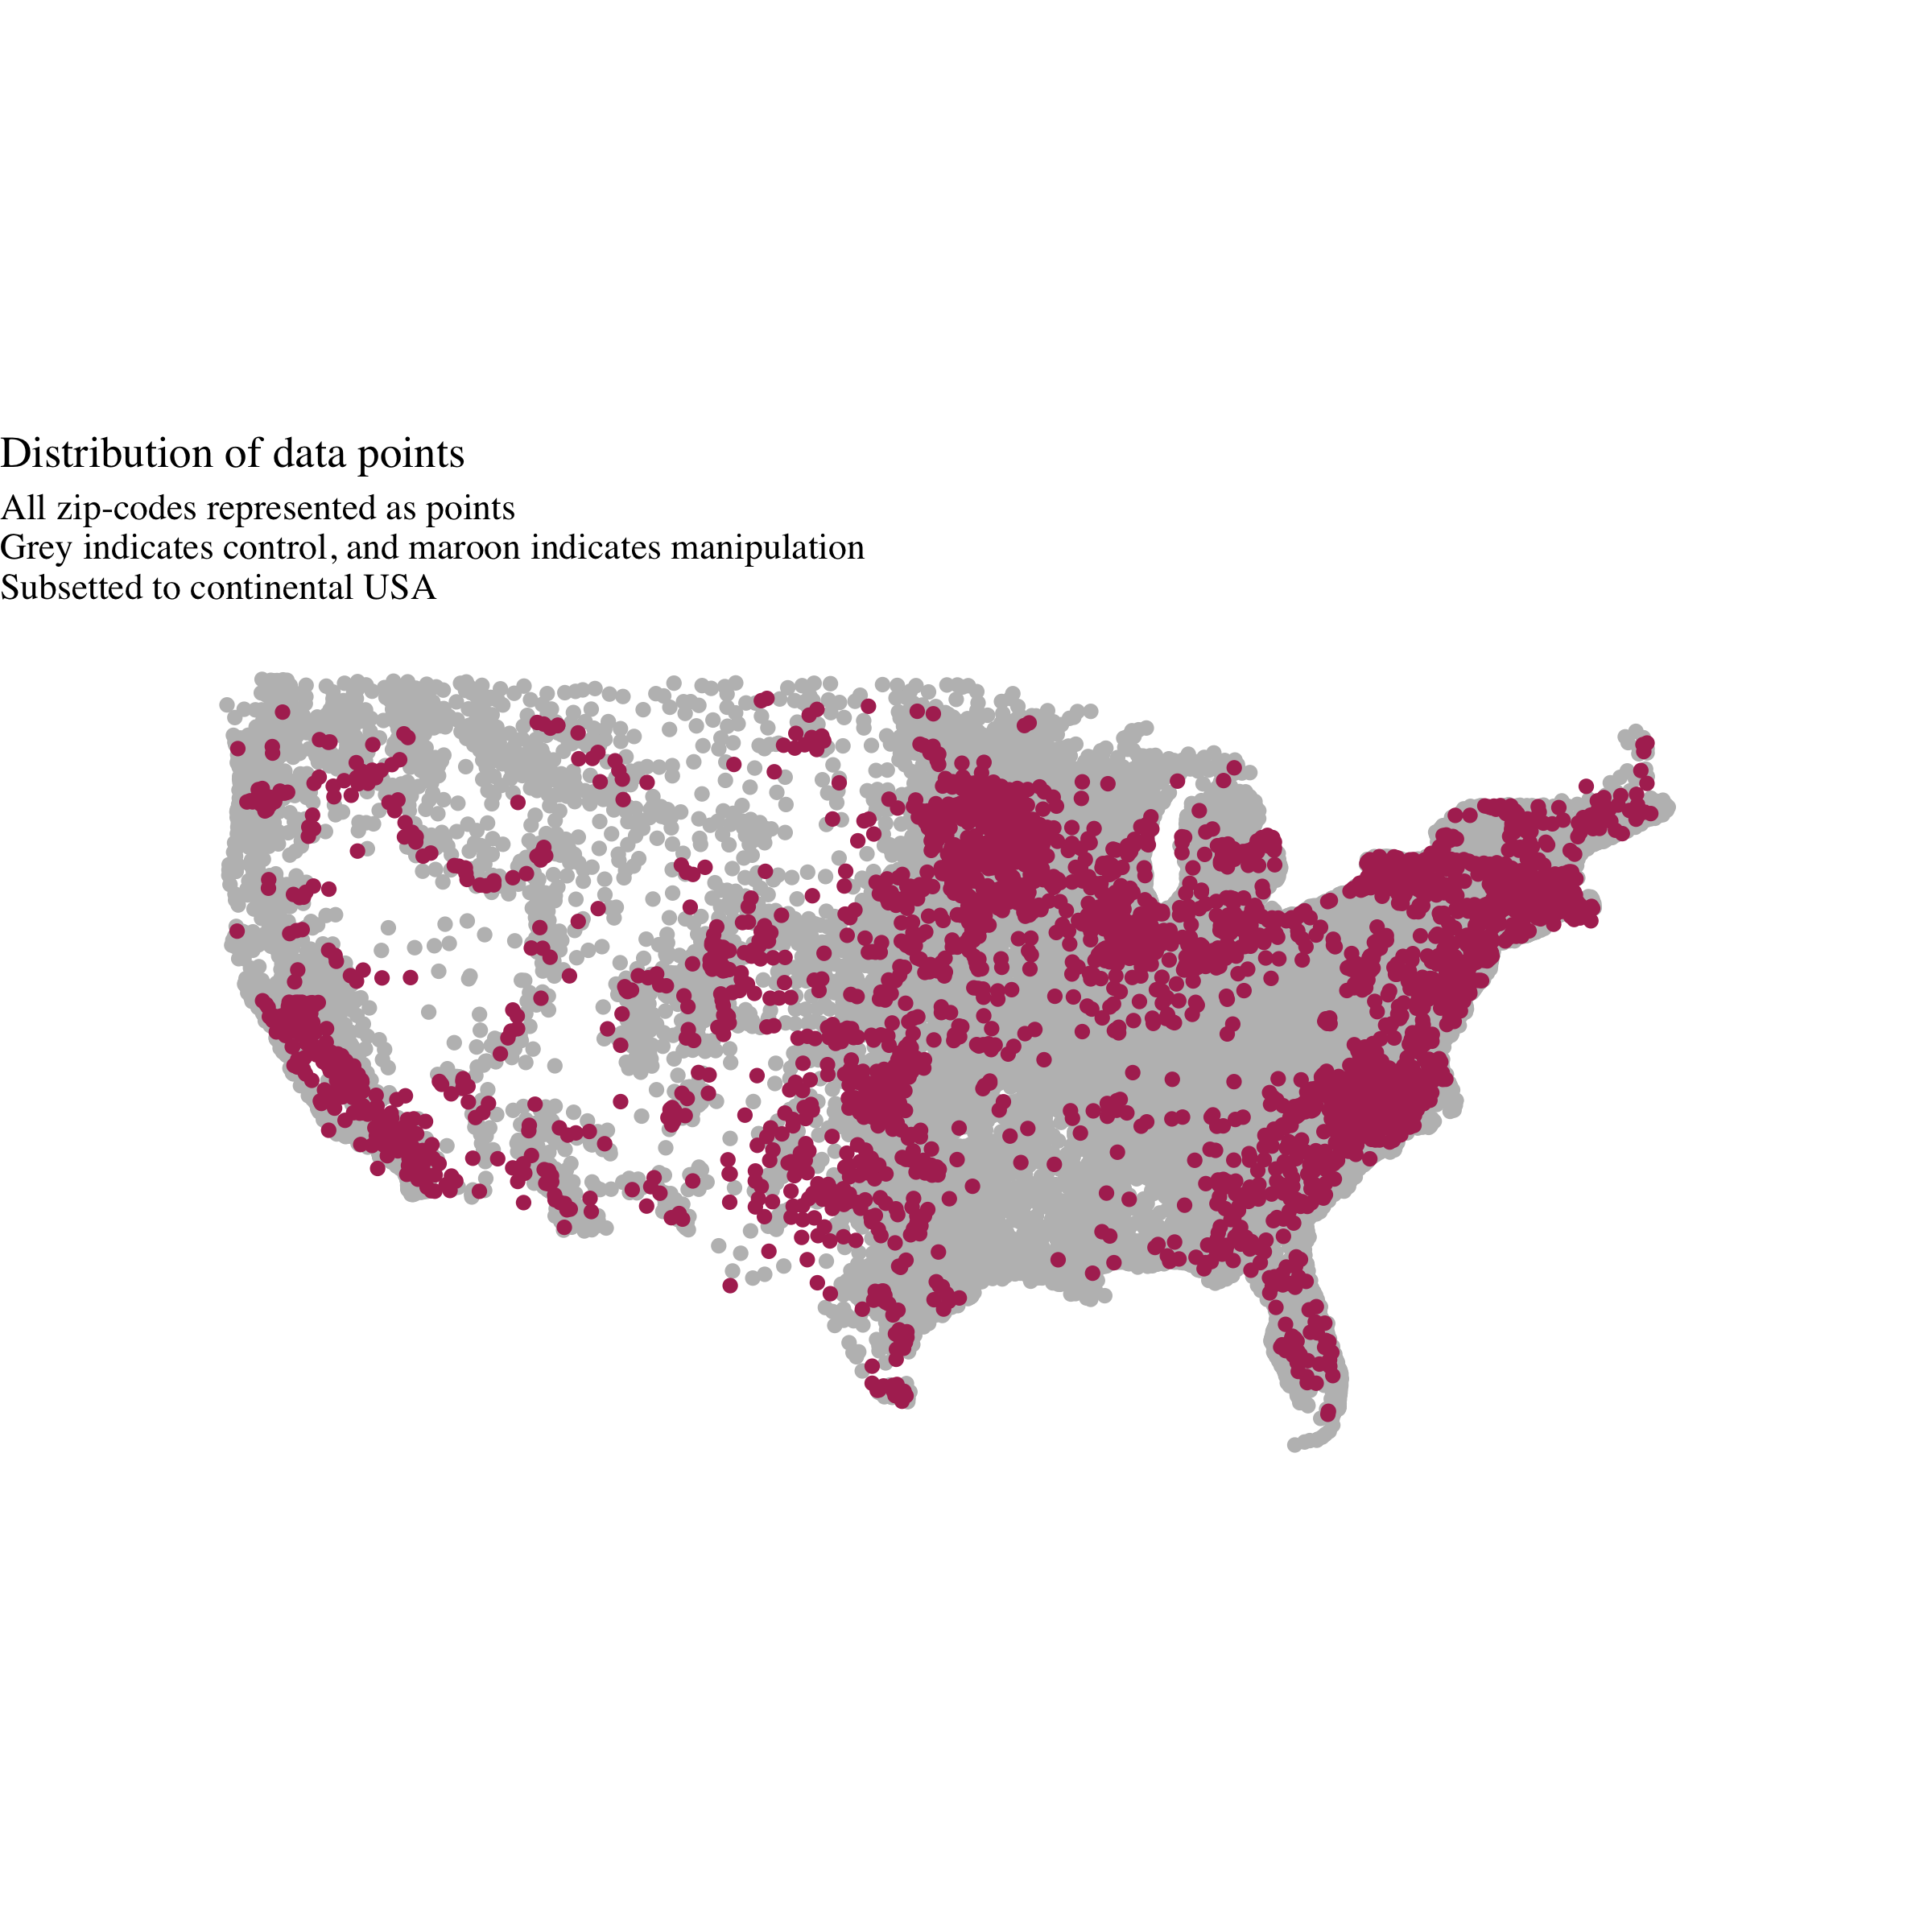
\includegraphics[width=0.9\linewidth]
{zip_code_centroids_continental.png} 
\caption{Distribution of zip-code centroids in the USA, zoomed in to the continental states}
\label{zips_continental}
\end{figure}

\begin{figure}[h]
\centering
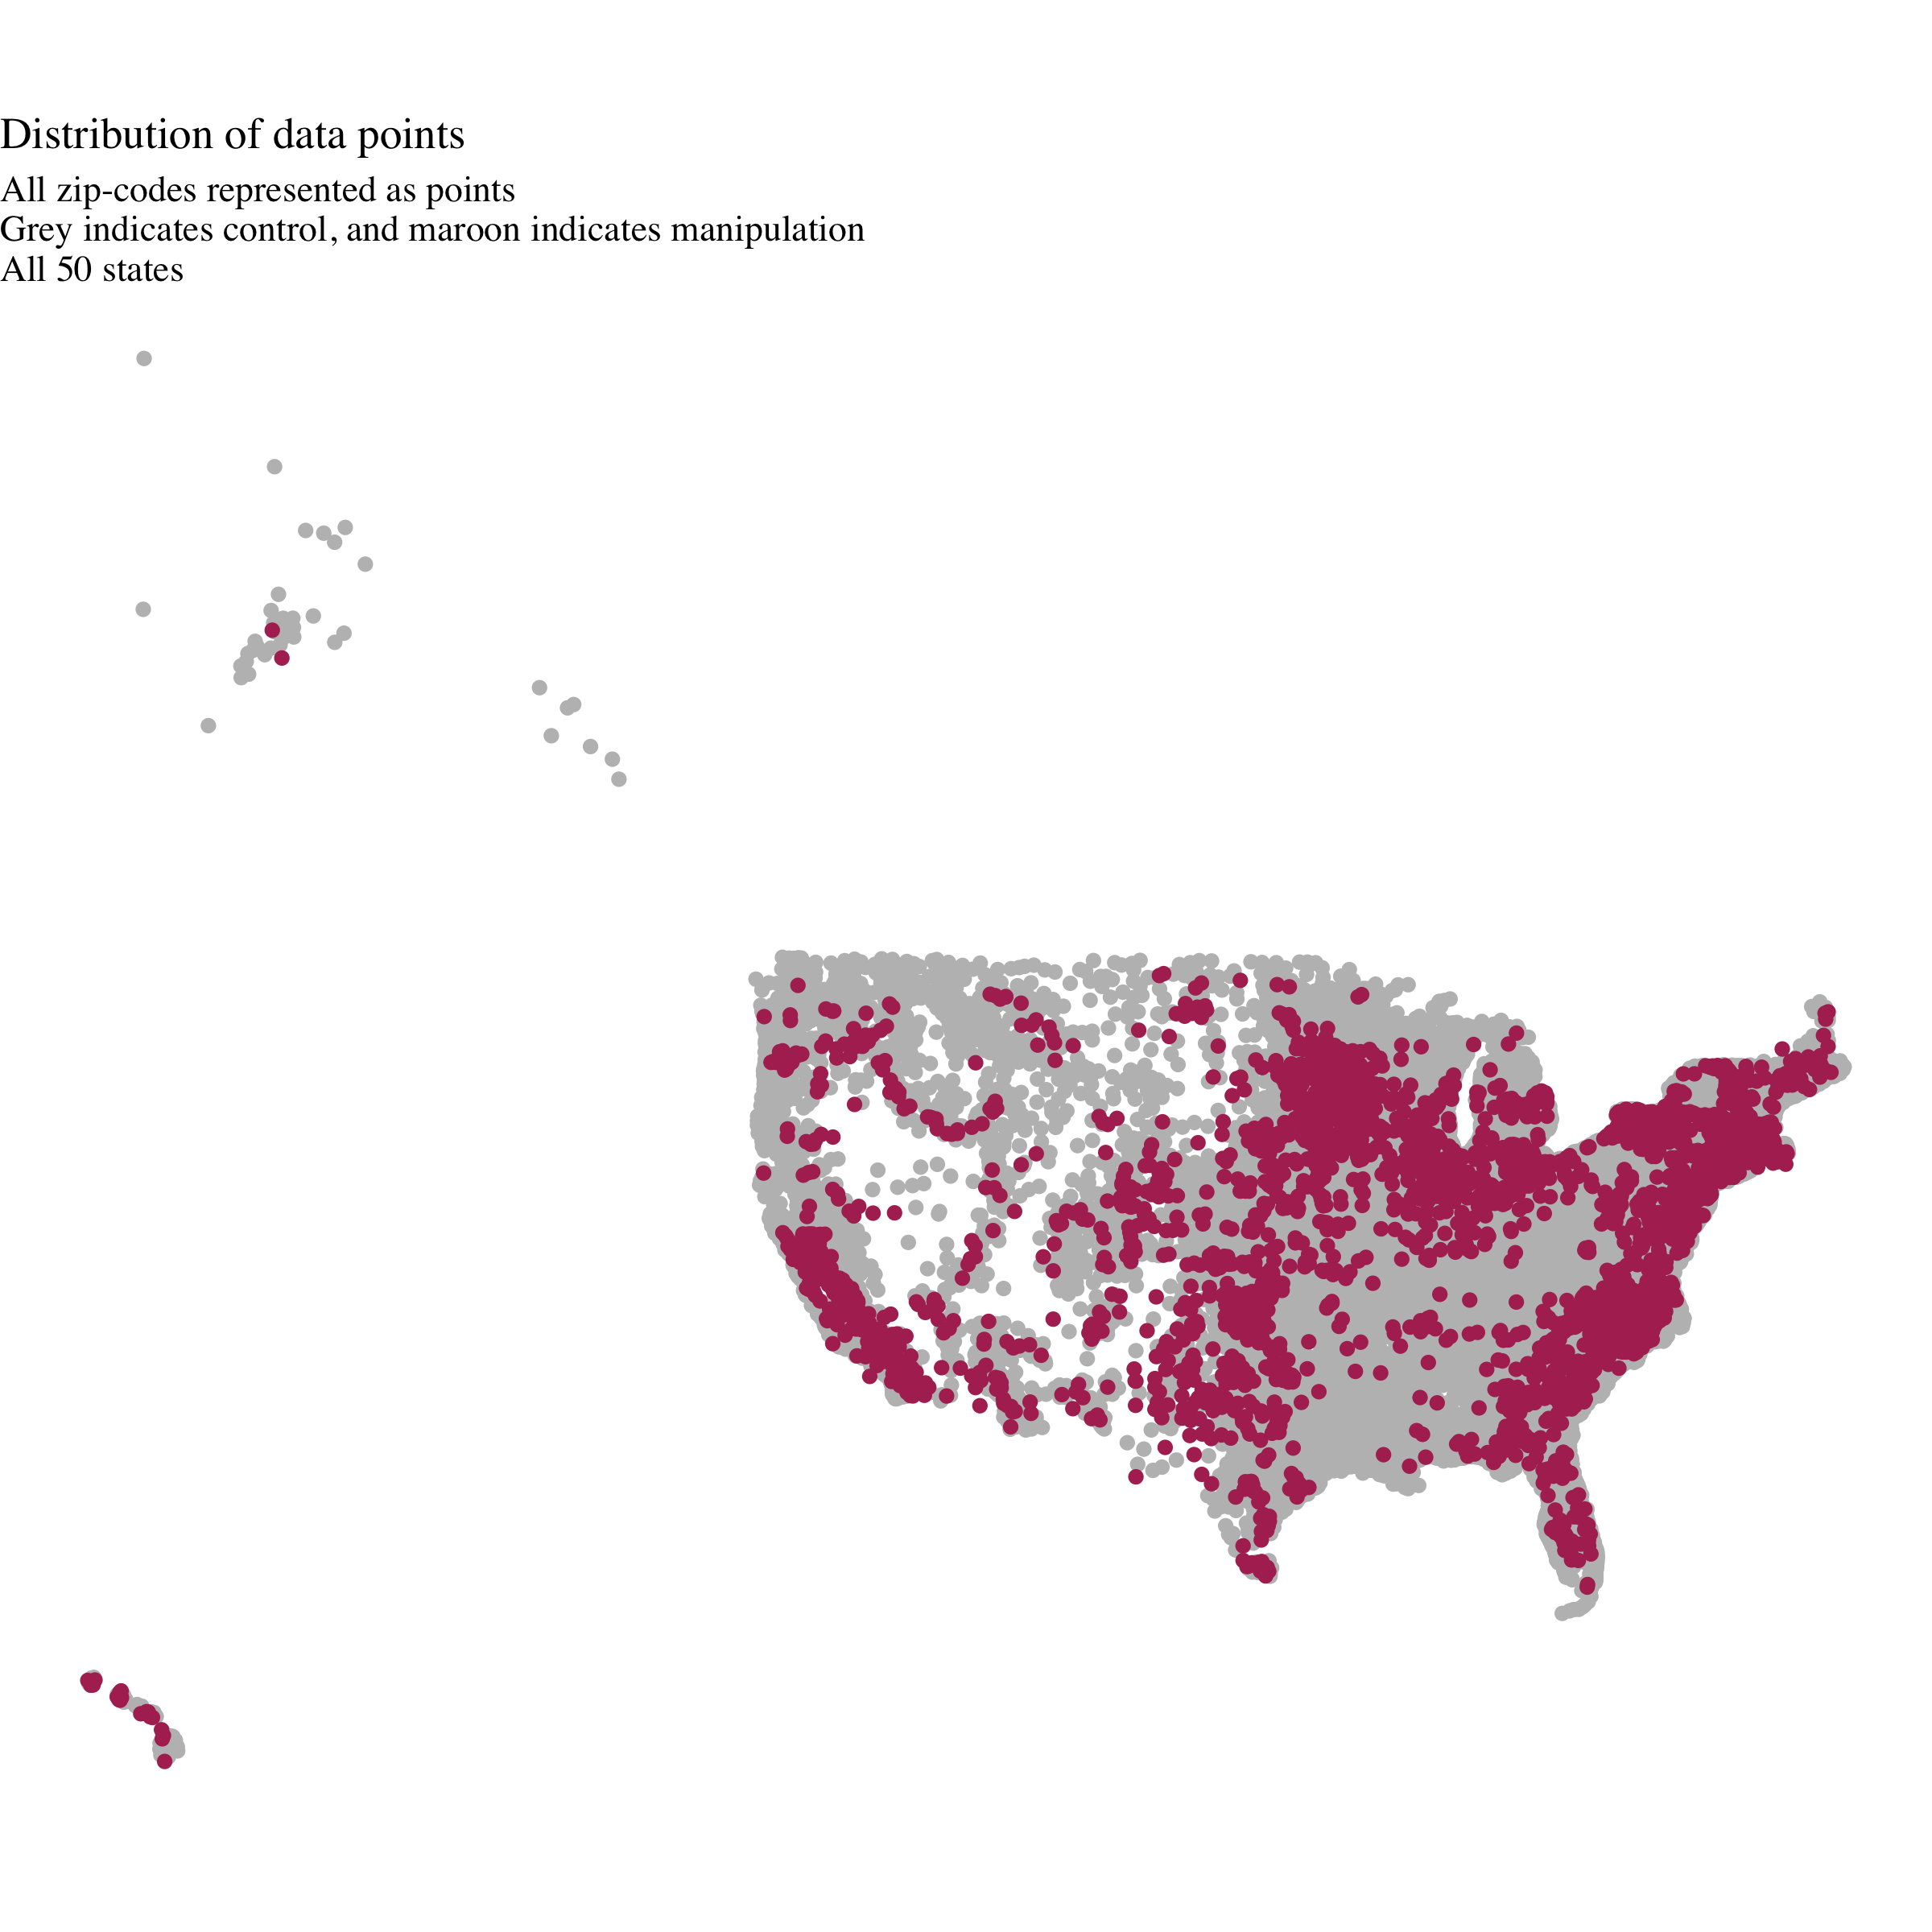
\includegraphics[width=0.9\linewidth]
{zip_code_centroids_all.png} 
\caption{Distribution of zip-code centroids in the USA, zoomed out. Alaska and Hawaii are included, but overseas territories are not represented in our dataset}
\label{zips_all}
\end{figure}


A cursory look at the distribution of our zip-codes indicates that we have both control and manipulation observations all over the USA (cf figures \ref{zips_continental} and \ref{zips_all}).
A further study would might take a step further than a cursory look, of course, and ensure that our data points are not biased in any way (eg over-sampling in certain states, in metropolitan vs rural areas, etc).


\section{Mixed-Effects Model}

The formula for our mixed-effects model is:
\begin{verbatim}
rate of home appreciation ~ 
\end{verbatim}
\begin{verbatim}
year + solar_manipulation + turbine_manipulation + (1|zip_code)
\end{verbatim}

\textbf{Dependent variable}
\begin{itemize}
\item The rate of home appreciation is calculated as: \emph{(current home price - last year's home price) / (last year's home price).}
\end{itemize}

\textbf{Fixed effects}
\begin{itemize}
\item Year: the calendar year, represented as an unordered factor. This allows us to easily represent general market fluctuations (eg the Great Recession around 2008).
\item Solar manipulation: if a zip code has a solar plant built there before 2024 (the end of our Zillow dataset), then we want to classify each year vis-a-vis the solar plant construction. 
	\begin{itemize}
	\item Construction: if only one solar plant is built in this zip-code, then `construction' is synonymous with `year of operation'. If multiple solar plants are built in this zip-code, this represents the duration between the first plant's year of operation and the last plant's year of operation. Since I don't make assumptions as to how long a given project took to build, I use `construction' as a catch-all for a period when I have faith that someone was tinkering around with wrenches and trucks
	\item -5, -4, -3, -2, -1: Years prior to the construction period
	\item 1, 2, 3, 4, 5: Years after the construction period
	\item Censored: Any year either more than five years before the construction period, or more than five years after the construction period
	\item Control: a zip-code that never gets a solar project
	\end{itemize}
\item Turbine manipulation: encoded exactly like solar manipulation
\end{itemize}
\textbf{Random effects}
\begin{itemize}
\item Zip-code: here, I model all zip-codes as random intercepts. This is a common practice in models that have repeated measures per subject; it compensates for the mean difference in home appreciation in each zip-code
\end{itemize}


\subsection{Goodness-of-Fit Metrics}
In order to verify whether it's even sensible to try to calculate the impact of green energy projects, we also fit a null model, which omits turbine manipulation and solar manipulation.
The null model's formula is:
\begin{verbatim}
rate of home appreciation ~ year + (1|zip_code)
\end{verbatim}
.

A chi-squared test comparing these two models indicates that the full model is statistically significant; 
${\chi}^2(23, N=471,142)=126.6, p < 0.01$
(see figure \ref{anova}).
This denotes that it is sensible to study the impact that the turbine and solar plants have on these zip-codes.

\begin{figure}[h]
\centering
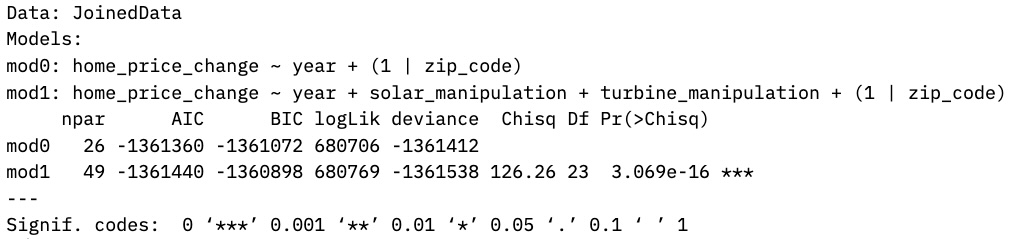
\includegraphics[width=0.9\linewidth]
{lmer_mod_anova.jpg} 
\caption{The full regression model is statistically significant, compared to the null model which omits green energy projects. This indicates that the impact of green energy projects is statistically significant.}
\label{anova}
\end{figure}

The unadjusted intra-class correlation (\emph{ICC}) in our full model is 0.011, which is quite low.
A high ICC would indicate that the random effects are explaining a lot of the variance in our full model.
We don't want this; we want what we see, which is that our fixed effects are explaining a lot of the variance. 

\subsection{Estimates}

The fixed effects can be visualized in figure \ref{fixef_general} and figure \ref{fixef_manipulation}, but they are listed below in their entirety.
For each fixed-effect variable, you can see both the estimate, and the 95\% confidence interval.
If any confidence interval includes 0.0, then it's reasonable to say that this variable is statistically insignificant.

\begin{table}[]

\small

\begin{tabular}{llll}
\textbf{Variable}                 & \textbf{Estimate} & \textbf{2.5\%} & \textbf{97.5\%} \\
(Intercept)                       & 0.053             & 0.047          & 0.058           \\
year2002                          & 0.015             & 0.013          & 0.016           \\
year2003                          & 0.014             & 0.013          & 0.015           \\
year2004                          & 0.021             & 0.02           & 0.023           \\
year2005                          & 0.047             & 0.046          & 0.049           \\
year2006                          & 0.05              & 0.049          & 0.052           \\
year2007                          & -0.013            & -0.014         & -0.012          \\
year2008                          & -0.071            & -0.072         & -0.069          \\
year2009                          & -0.131            & -0.132         & -0.13           \\
year2010                          & -0.116            & -0.117         & -0.115          \\
year2011                          & -0.09             & -0.091         & -0.089          \\
year2012                          & -0.097            & -0.098         & -0.096          \\
year2013                          & -0.029            & -0.031         & -0.028          \\
year2014                          & 0.005             & 0.004          & 0.006           \\
year2015                          & -0.012            & -0.013         & -0.01           \\
year2016                          & 0.001             & -0             & 0.002           \\
year2017                          & -0.014            & -0.016         & -0.013          \\
year2018                          & -0.003            & -0.004         & -0.002          \\
year2019                          & -0.003            & -0.004         & -0.002          \\
year2020                          & -0.006            & -0.008         & -0.005          \\
year2021                          & 0.055             & 0.054          & 0.057           \\
year2022                          & 0.082             & 0.081          & 0.083           \\
year2023                          & 0.015             & 0.014          & 0.016           \\
year2024                          & -0.03             & -0.031         & -0.029          \\
solar\_manipulation-2             & -0.001            & -0.004         & 0.003           \\
solar\_manipulation-3             & -0.001            & -0.005         & 0.002           \\
solar\_manipulation-4             & -0.002            & -0.005         & 0.002           \\
solar\_manipulation-5             & -0.003            & -0.007         & 0.001           \\
solar\_manipulation1              & 0.004             & 0              & 0.007           \\
solar\_manipulation2              & 0.004             & 0              & 0.007           \\
solar\_manipulation3              & 0.006             & 0.003          & 0.01            \\
solar\_manipulation4              & 0.01              & 0.006          & 0.014           \\
solar\_manipulation5              & 0.009             & 0.005          & 0.013           \\
solar\_manipulationCensored       & 0.004             & 0.001          & 0.006           \\
solar\_manipulationConstruction   & 0.003             & -0             & 0.006           \\
solar\_manipulationControl        & 0.006             & 0.001          & 0.011           \\
turbine\_manipulation-2           & 0                 & -0.006         & 0.007           \\
turbine\_manipulation-3           & 0                 & -0.006         & 0.007           \\
turbine\_manipulation-4           & 0.001             & -0.006         & 0.007           \\
turbine\_manipulation-5           & 0.001             & -0.006         & 0.008           \\
turbine\_manipulation1            & -0.001            & -0.007         & 0.004           \\
turbine\_manipulation2            & -0.004            & -0.01          & 0.002           \\
turbine\_manipulation3            & -0                & -0.006         & 0.006           \\
turbine\_manipulation4            & 0                 & -0.006         & 0.006           \\
turbine\_manipulation5            & -0.003            & -0.009         & 0.004           \\
turbine\_manipulationCensored     & 0.003             & -0.002         & 0.008           \\
turbine\_manipulationConstruction & 0.002             & -0.003         & 0.007          
\end{tabular}
\caption{The estimates and 95\% confidence intervals for our fixed-effects}

\end{table}

Do note that while this model gives quite sensible estimates, we suffer from a relatively low sample size for a model of this complexity.
We have 412,303 observations in our control group, and only 58,839 in our manipulation group.
For this reason, this model was slightly rank-deficient.
(One notable missing value is turbine manipulation for the year just before operation.)

\begin{figure}[h]
\centering
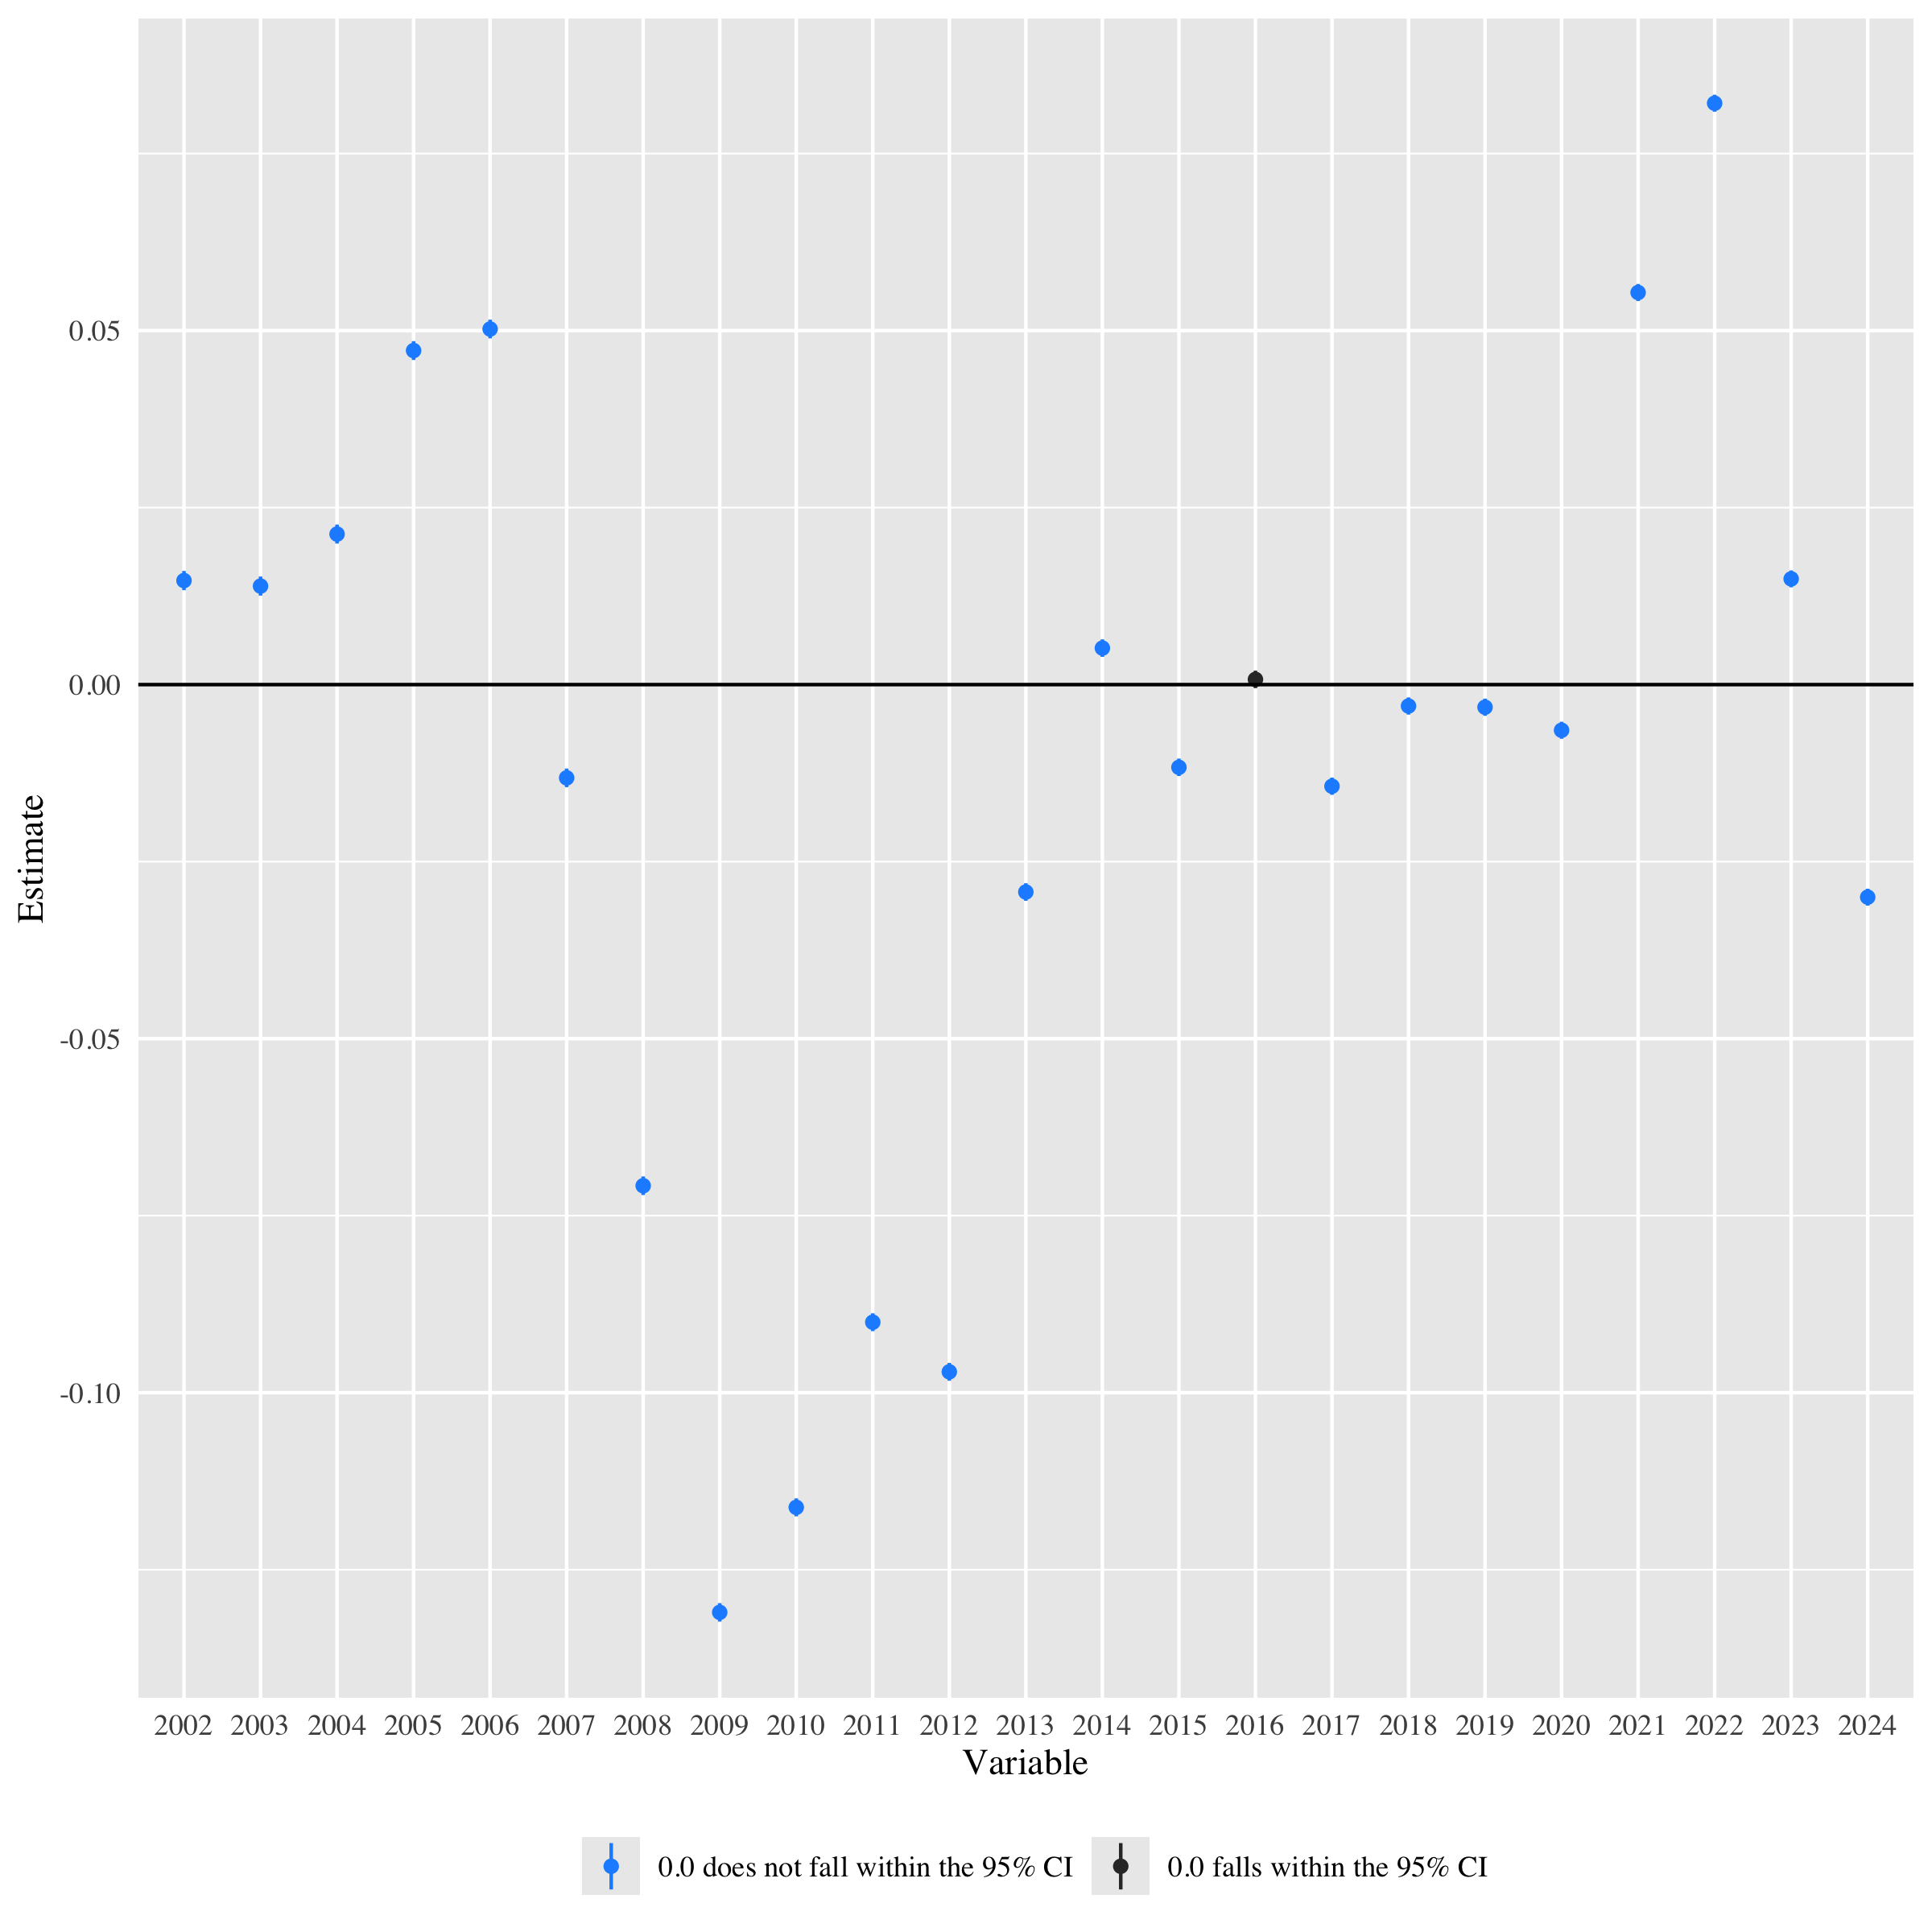
\includegraphics[width=0.9\linewidth]
{fixef_general.png} 
\caption{The yearly fixed-effects from the full model.}
\label{fixef_general}
\end{figure}

\begin{figure}[h]
\centering
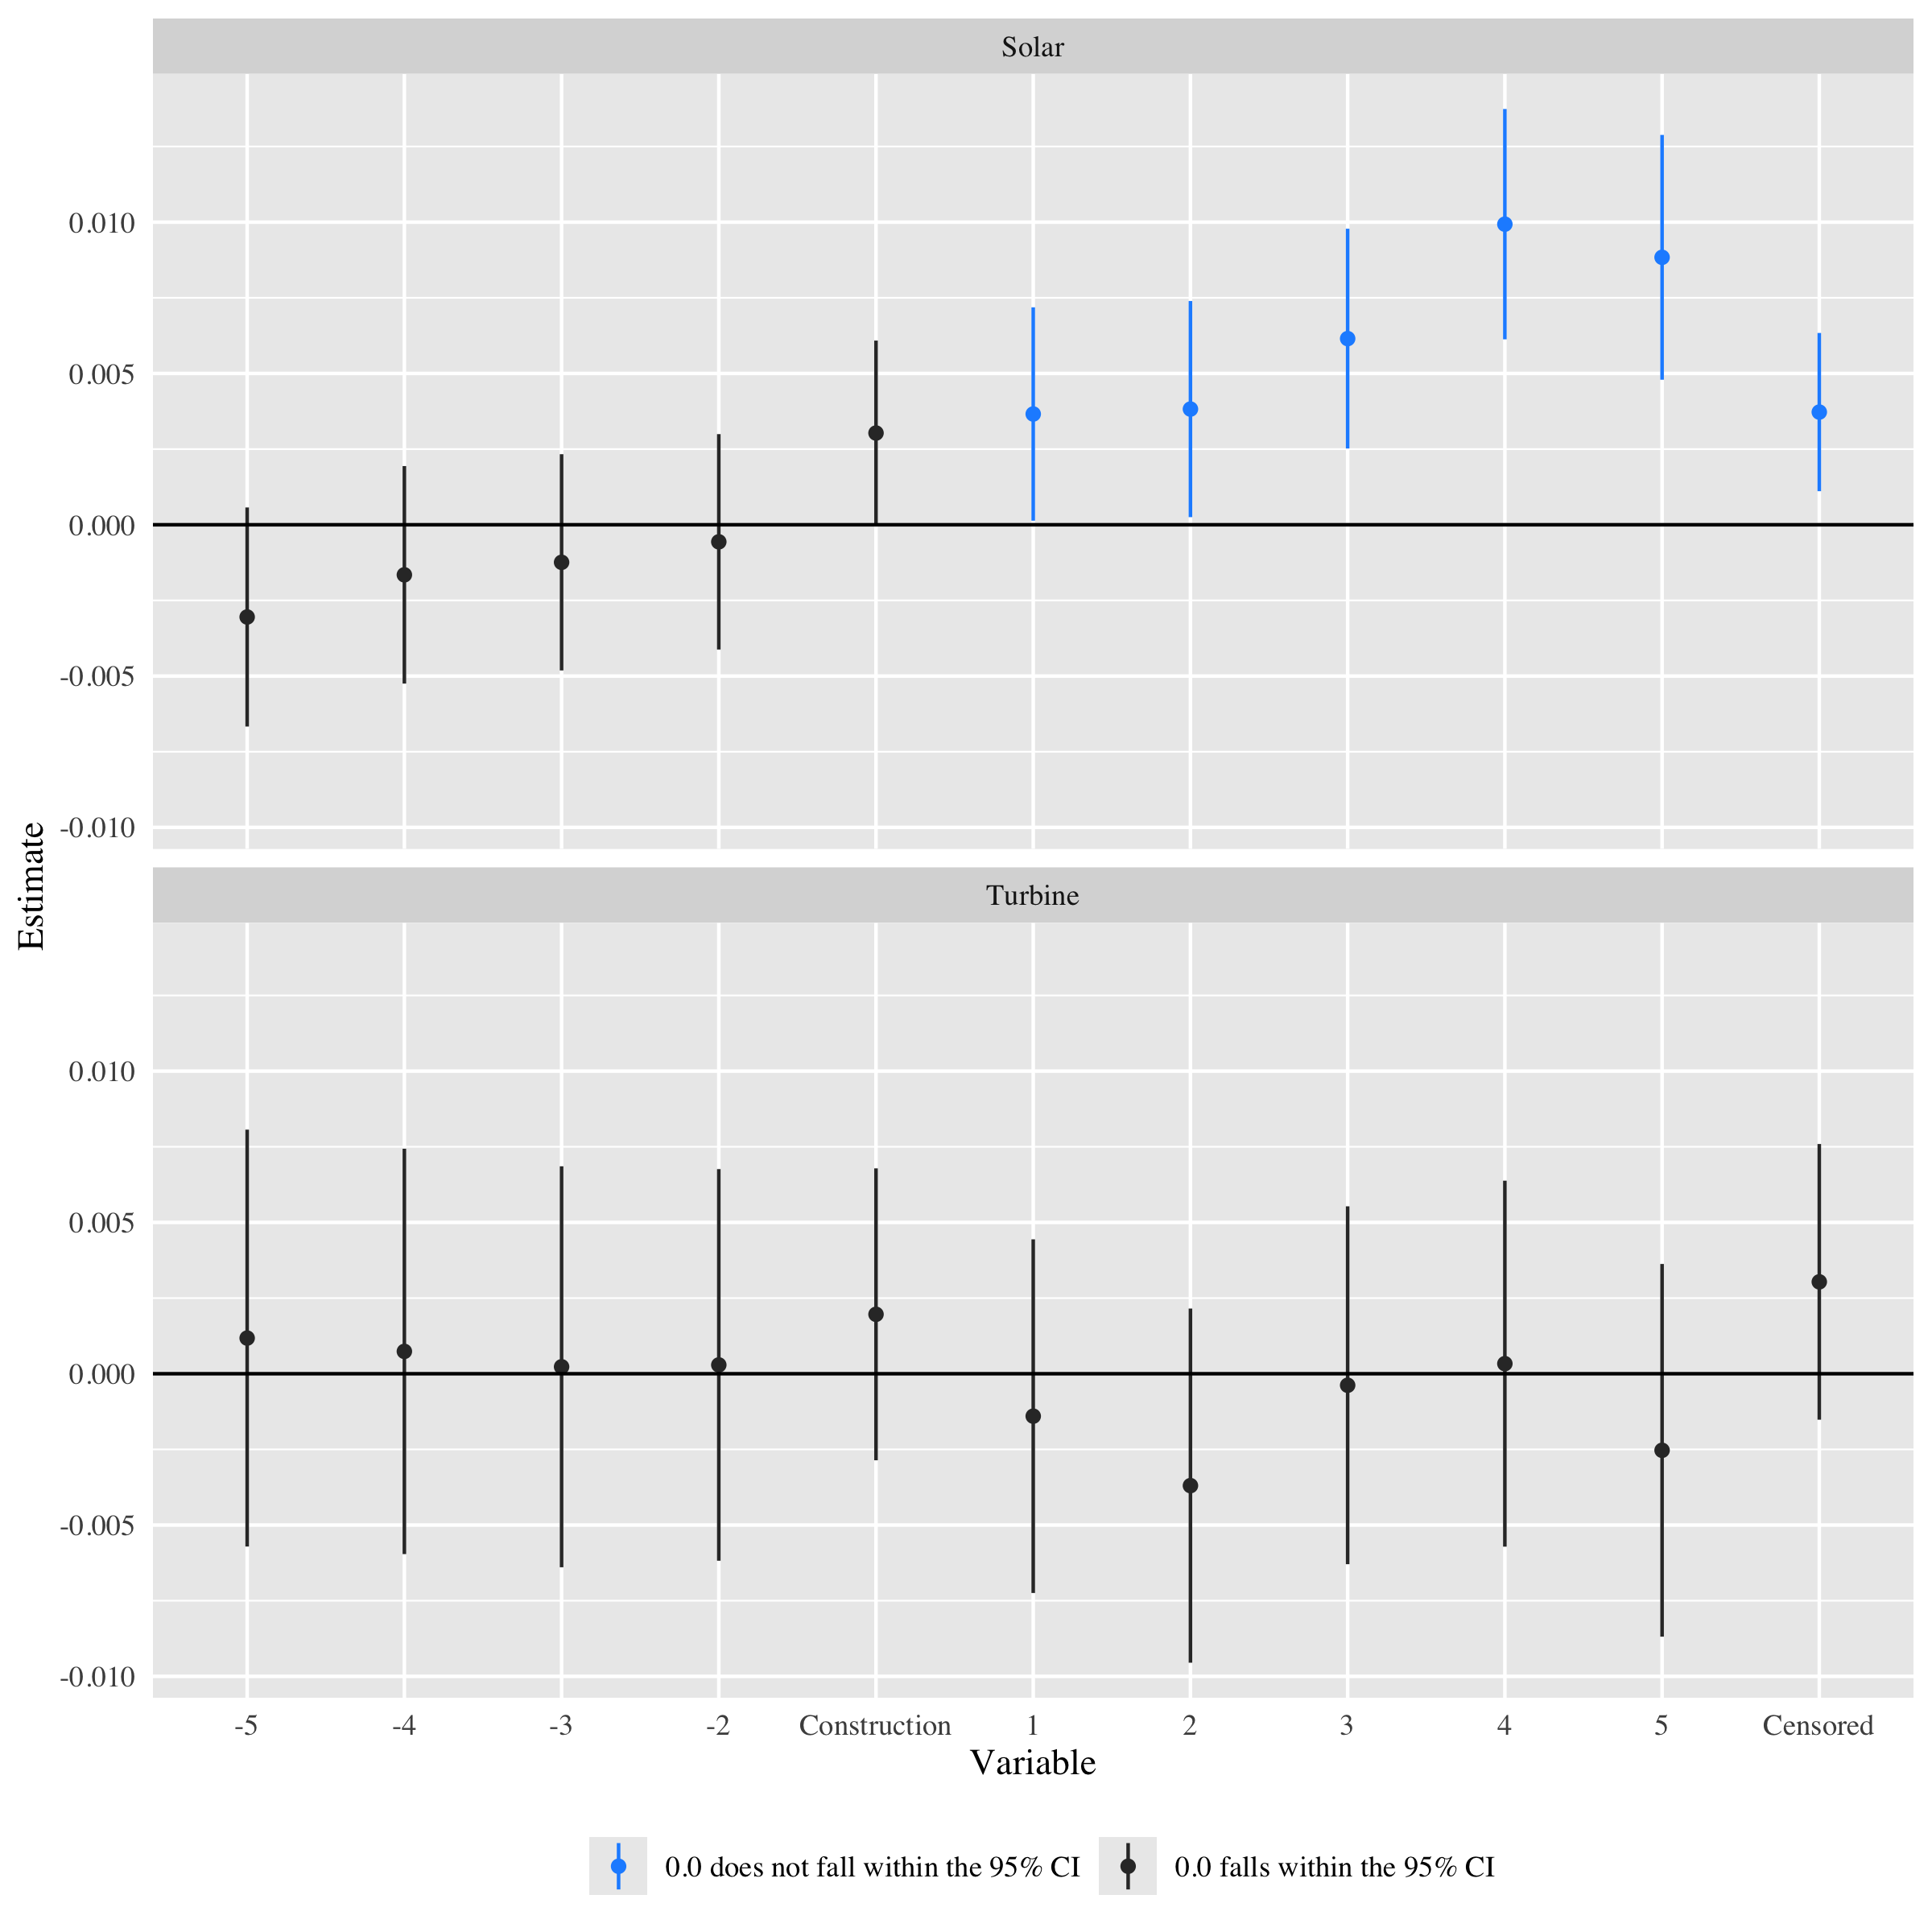
\includegraphics[width=0.9\linewidth]
{fixef_manipulation.png} 
\caption{The manipulation fixed-effects from the full model}
\label{fixef_manipulation}
\end{figure}

Figure \ref{fixef_general} shows the estimated coefficients for overall home appreciation for each calendar year.
Figure \ref{fixef_manipulation} shows the estimated coefficients for the impact of our manipulations.
Bearing in mind that \emph{these fixed-effects don't reflect home prices per se, but rather, the rates at which home-prices change} given different situations, I interpret these in the following way:
\begin{itemize}
\item We can posit that any fixed-effect whose 95\% confidence interval includes zero does not significantly differ from no effect at all. 
Consequently, we can't really glean too much from  most of the trends that we see in the solar and turbine figure (figure \ref{fixef_manipulation}), because their CIs generally contain zero. 
On the other hand, our dataset is kind of small for this kind of model, and we have scant few manipulation observations compared to the control observations.
We can see evidence of this small sample size/imbalance in the very slim 95\% CIs in the yearly fixed-effects, compared to the large ones in the manipulations; this might be because we have so many more observations in our control set than in our manipulation set. 
\emph{I suggest we cautiously try to make sense of the manipulation estimates, while acknowledging that without a larger dataset, our interpretations are speculative.}
\item The only estimates whose CIs don't include zero are the solar estimates, in the years after the construction is done, and in the `censored' period (ie greater than five years away from construction, either before or after). 
It is possible that these positive estimates are actually evidence that just after the construction is over, the rate at which the house prices rise near solar plants increases, which allows them to regress back to their expected values, ceteris paribus.
I think this is a very promising research question: is the temporary decrease in the rate of home appreciation in zip-codes near solar facilities due to all the 'hubbub' of construction and the fear that the facility will be unsightly? and that once construction is over, the home values essentially return to normal, once people realize that it's not so bad to live near a solar facility?
I think this would be a really interesting follow-up study.

A note against my own interpretation: the fact that the 'censored' value is positive could challenge this hypothesis. This is because `censored' includes values both before and after construction. Positive censored estimates \emph{after} construction jibes with my theory; positive censored values \emph{before} construction challenge it. But in a model that is already rank-deficient, I can't really slice and dice our data much more to explore this.
\item Homes that are near construction sites appreciate in value slower than homes in control groups, which makes sense to me.
\item I wonder if the rates of appreciation for homes in zip-codes with turbines never fully rebound to the overall expected rate of home appreciation, because unlike solar plants, turbines make a bit of noise and are highly visible.
\end{itemize}


\section{Appendix}

I think the previous model is my best attempt to model this data.
However, a classic Difference-in-Difference comparison isn't done with a mixed-effects model-- it's done with a two-way fixed-effects model.
So, in order to honor convention, I model that as well.
I include it here in the appendix for your edification-- so you can see its results, and also, why I take issue with this model.

This model simplifies the previous model by simply asking if the rate of home appreciation changes over time differently in neighborhoods that \emph{do} have solar/turbines developed there versus in neighborhoods that \emph{don't}:
\begin{verbatim}
(past v present) x (manipulation v control)
\end{verbatim}

So, for any target year, I note all of the zip-codes where a single green energy project comes online in that target year.
Once again, rate of home appreciation is defined as:
\noindent\textit{(current home price - last year's home price) / (last year's home price). }
I track the rate of home appreciation in these manipulation zip-codes for 11 years-- the year of operation, the five years before, and the five years after.
I also track the rate of home appreciation in our control set, which remains all of the zip-codes in our Zillow dataset that never get a single green energy project built in it.

If the median rates of change in our control group differ from the median rates of change in our manipulation group, then we have a DiD trend that we can study!

Nota bene:
\begin{itemize}
\item Zip-codes with more than one green energy project are excluded from this study-- it's too complicated for a single model like this.
\item Perhaps if we have eleven observations representing the passage of time, this isn't exactly a two-way fixed-effect model?
\end{itemize}

\begin{figure}[h]
\centering
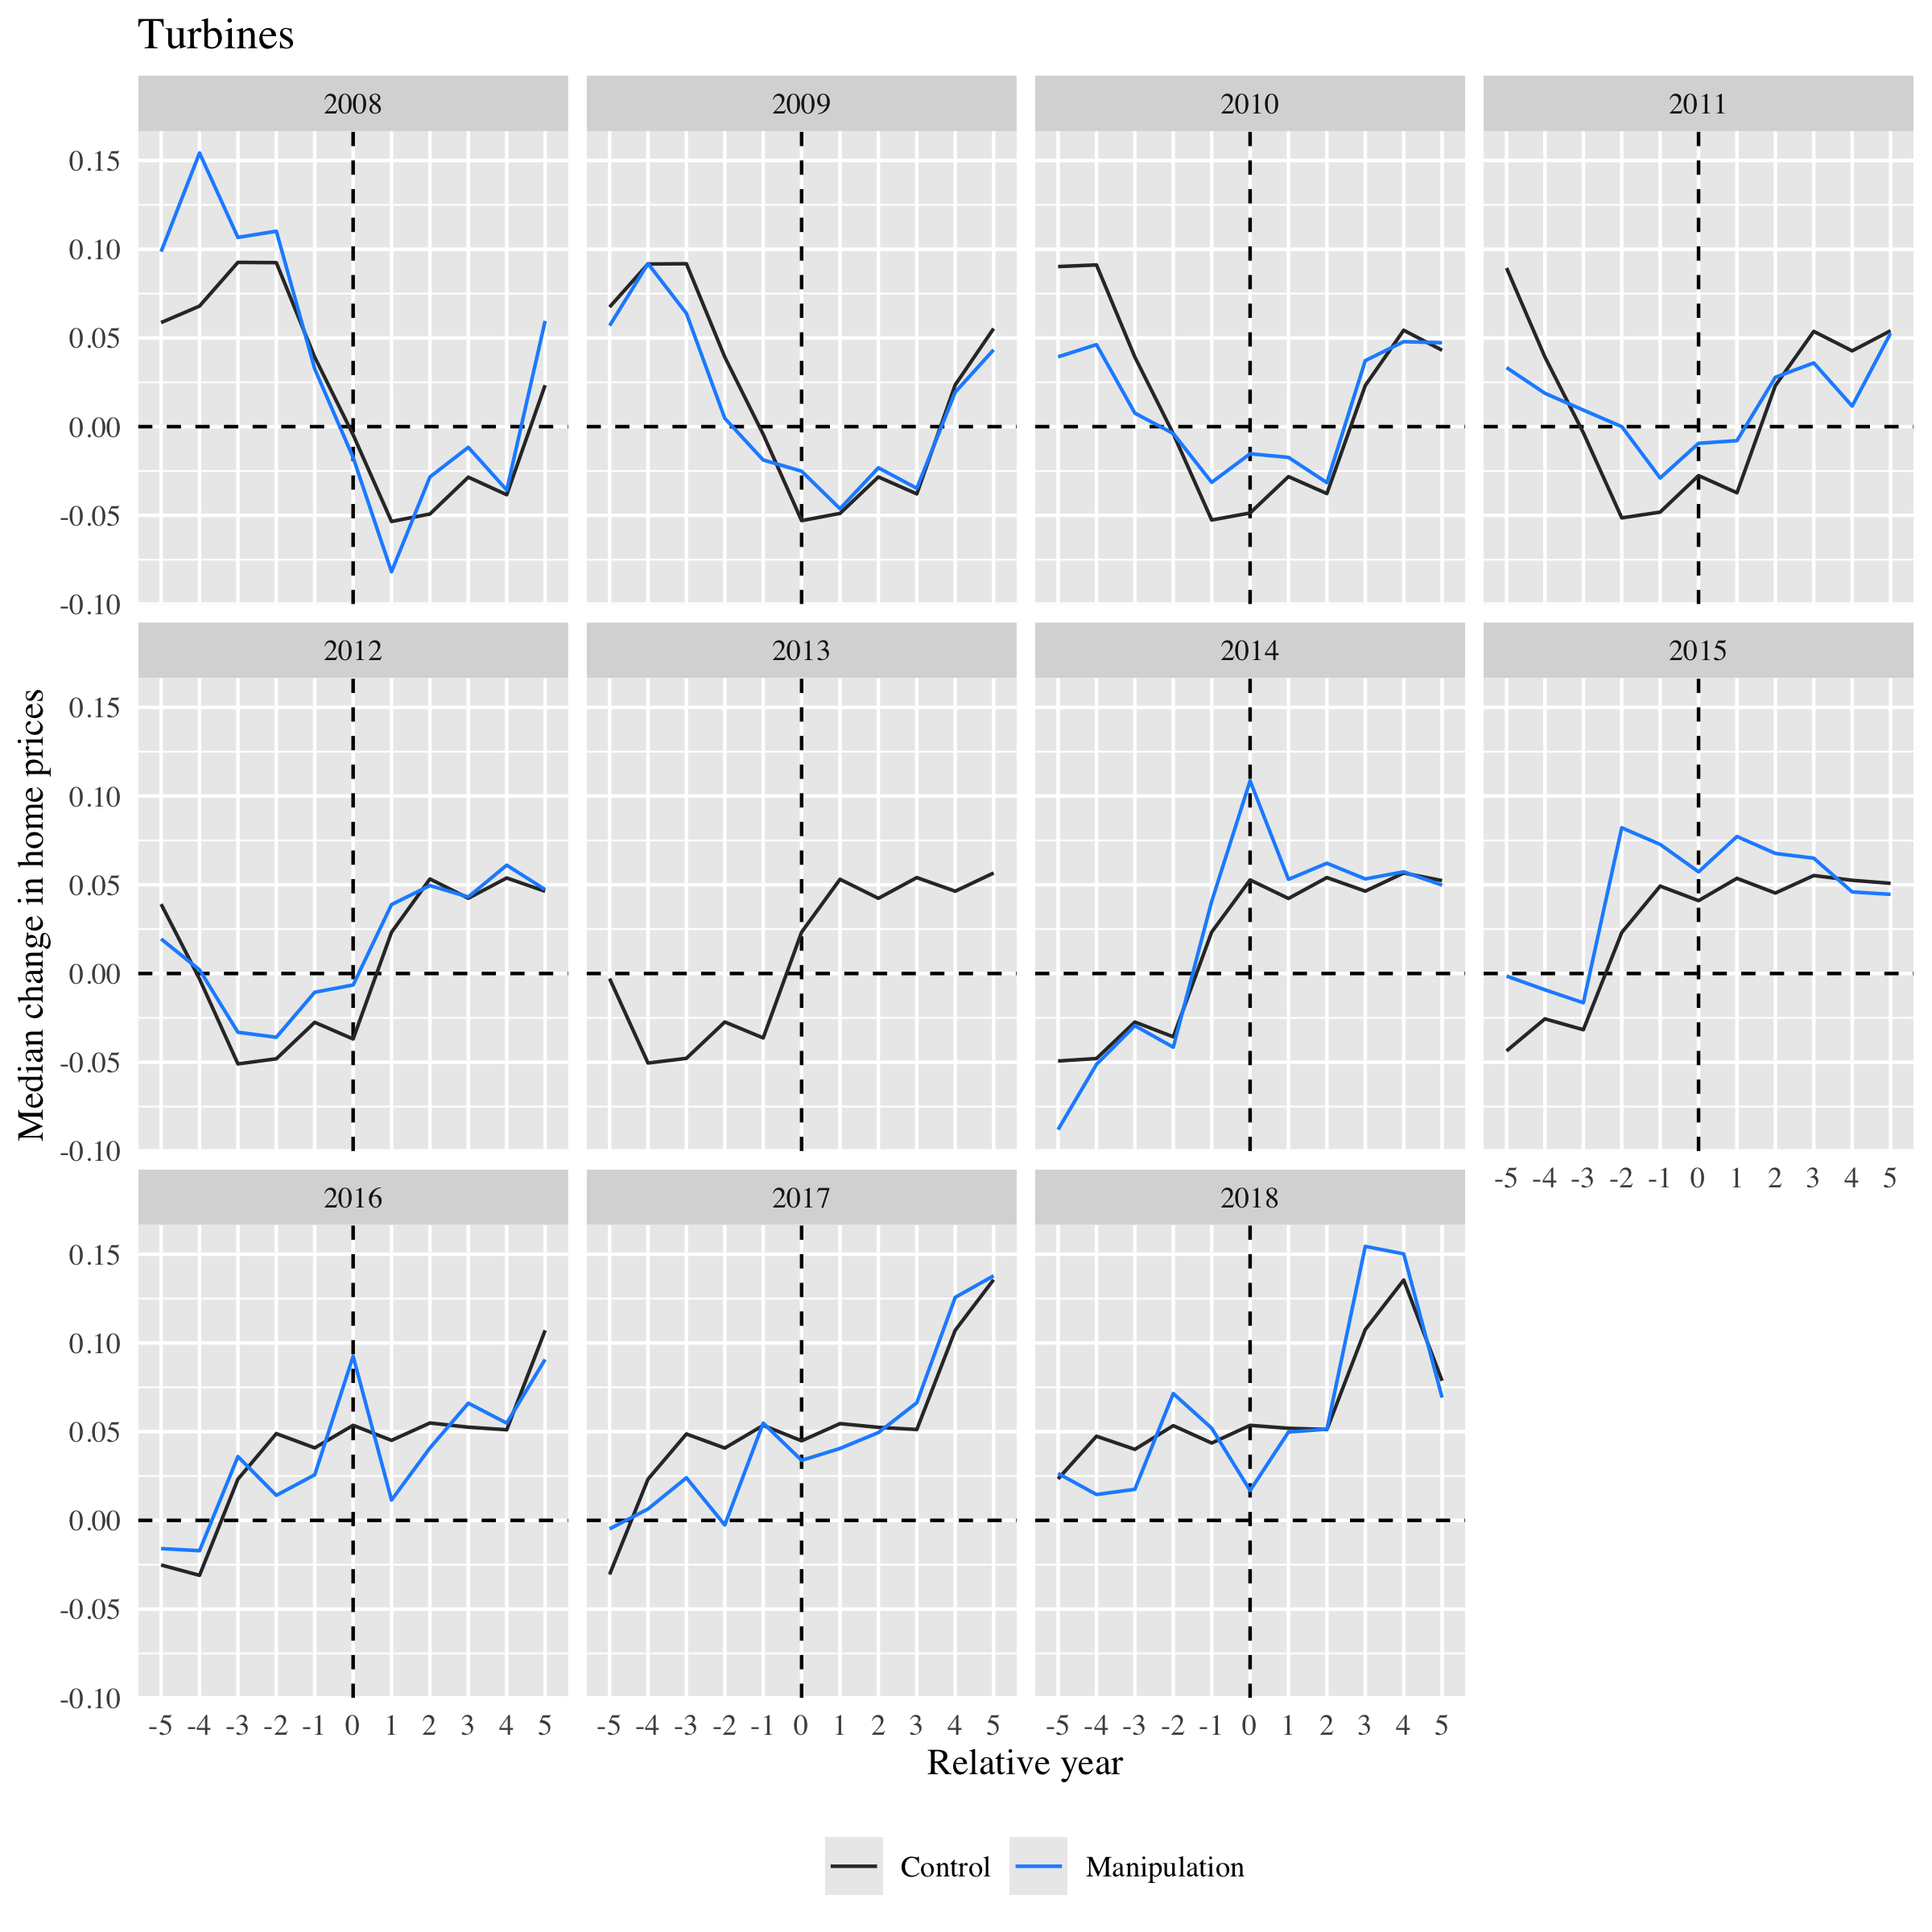
\includegraphics[width=0.9\linewidth]
{study1_turbine_facets.png} 
\caption{Median change in home prices in zip-codes that had wind turbines installed}
\label{study1turbinefacets}
\end{figure}

\begin{figure}[h]
\centering
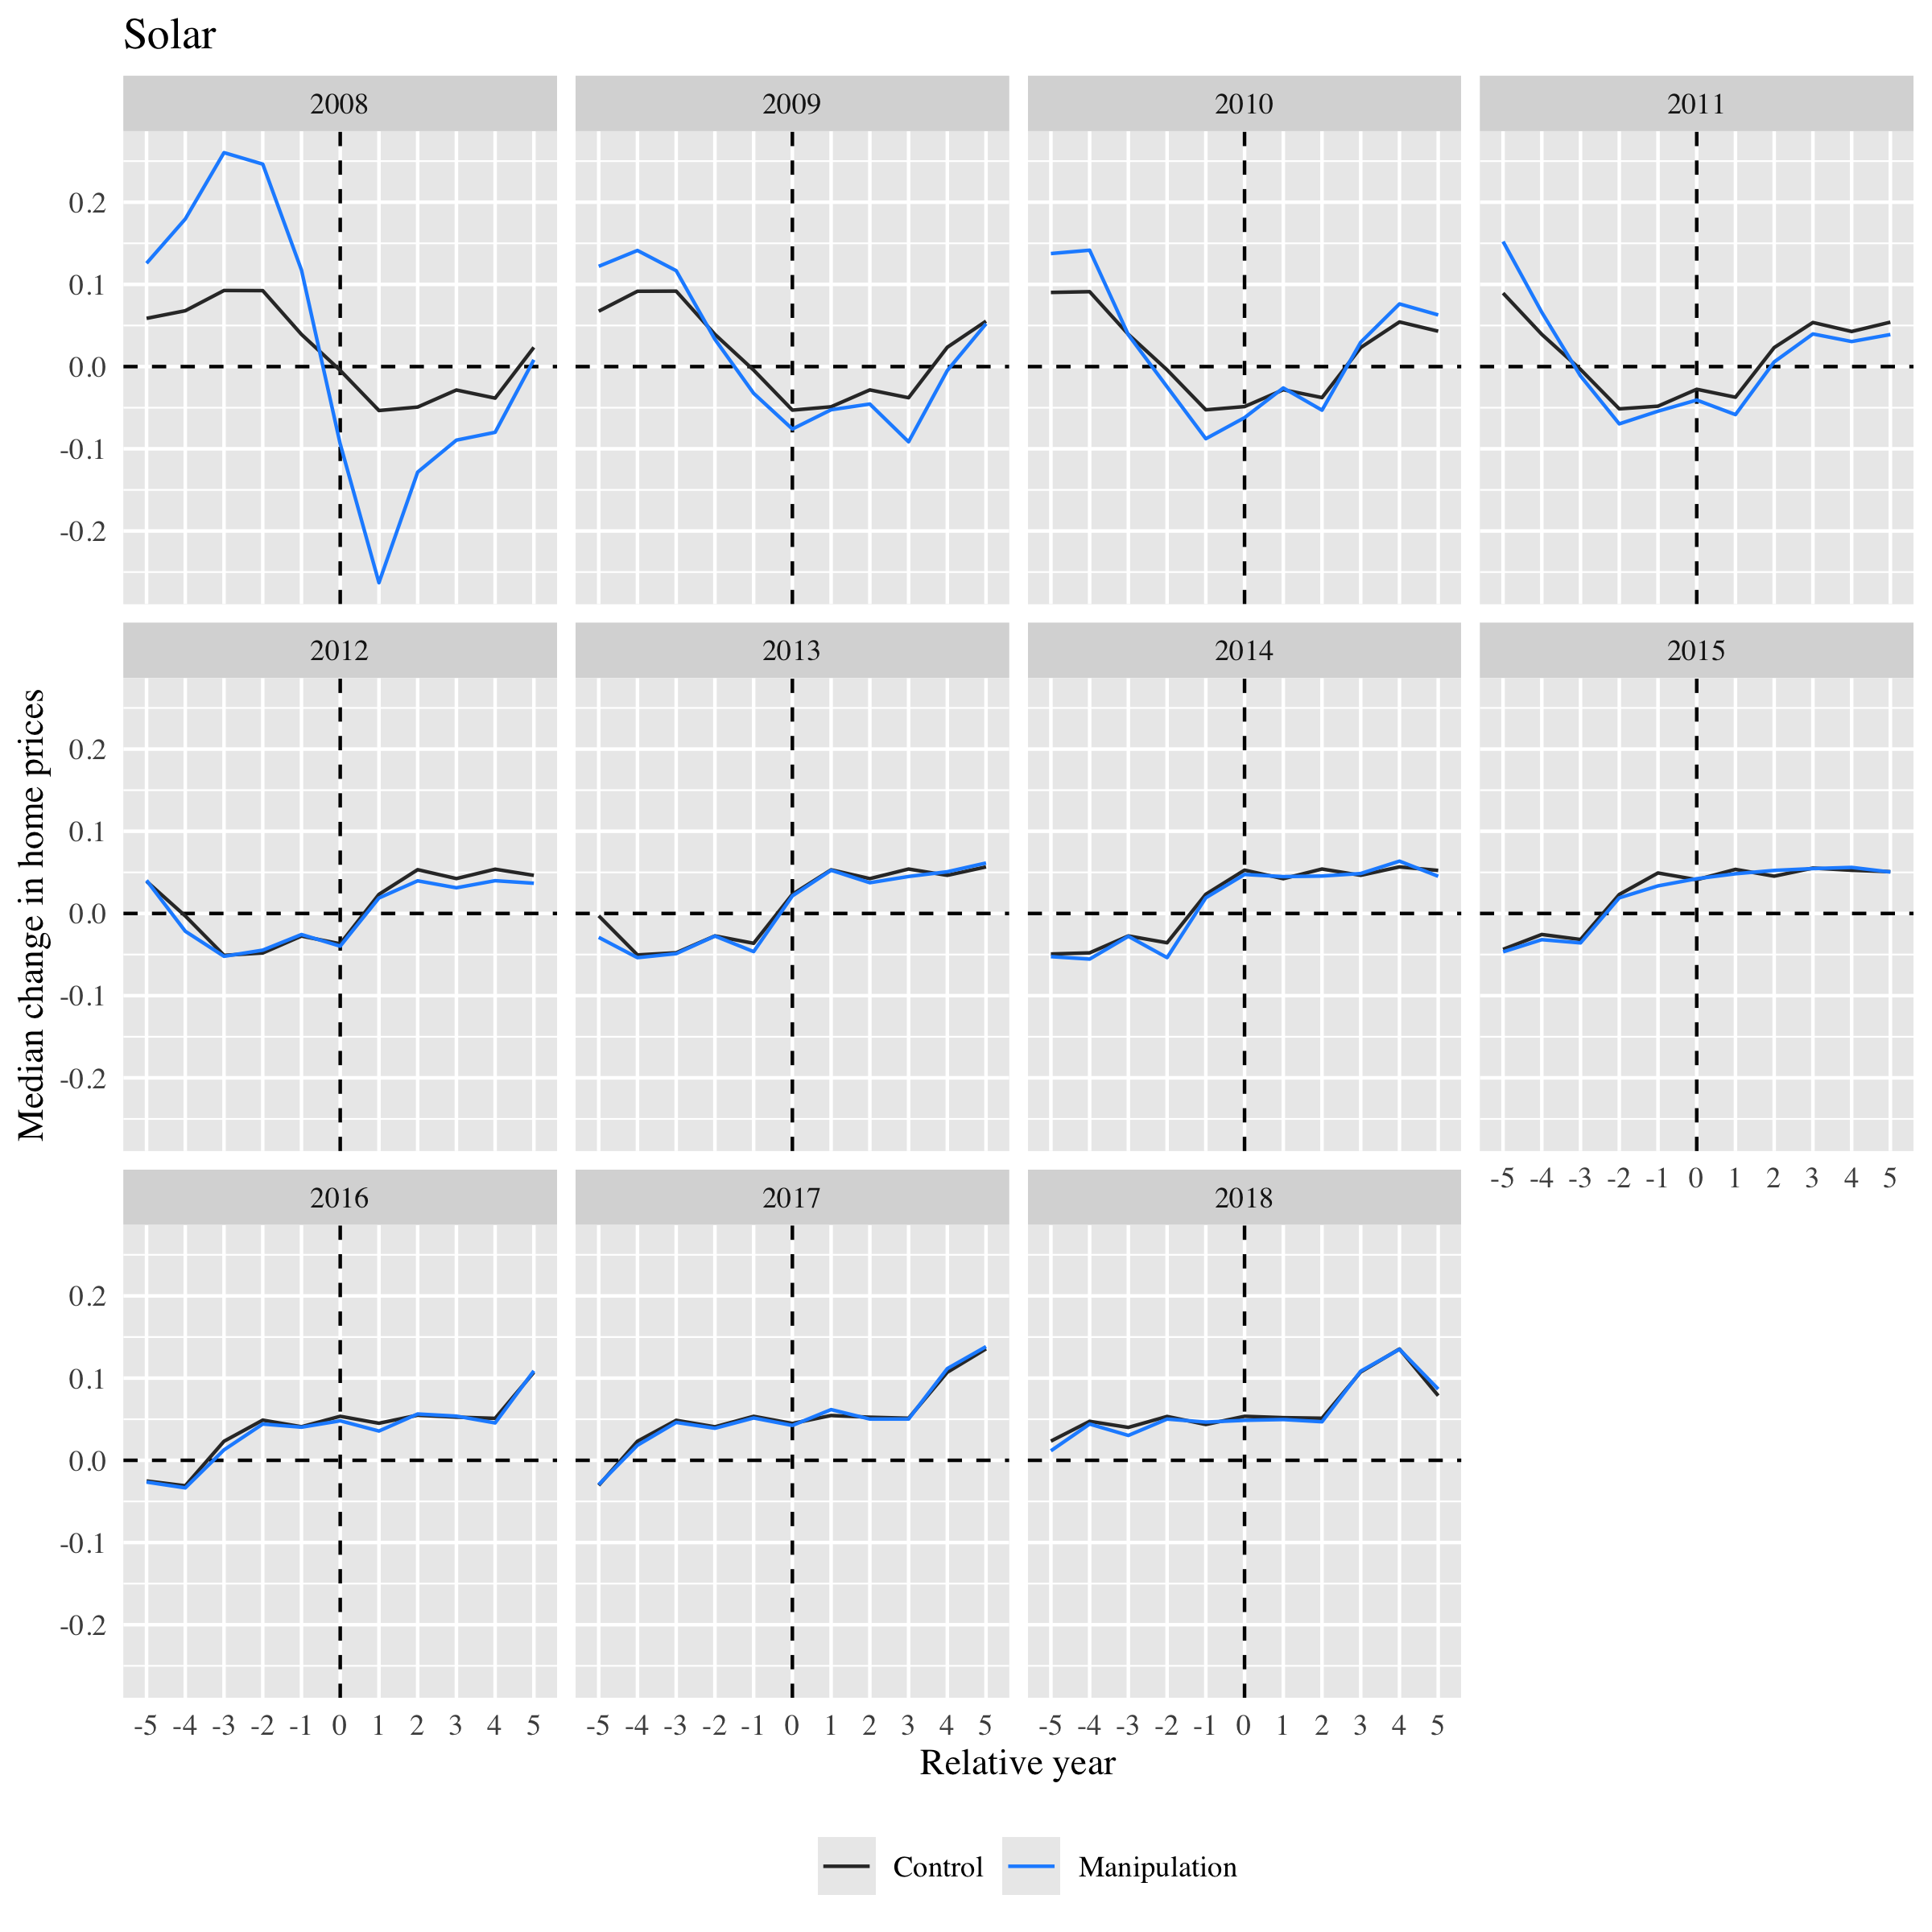
\includegraphics[width=0.9\linewidth]
{study1_solar_facets.png} 
\caption{Median change in home prices in zip-codes that had solar panels installed}
\label{study1solarfacets}
\end{figure}

You can see the results in figures \ref{study1turbinefacets} and \ref{study1solarfacets}, but I don't think there's many lessons to glean from these diagrams; these diagrams \emph{can't account for general changes in the real estate market.}
For example, we can see the market tanking in 2008, but this completely confounds our ability to compare these lines to those a decade later.

The other issue with this DiD study is, once again, a small sample size (see figure \ref{study1samplesize}). 
The sample sizes for the manipulation groups pictured here are very small, only a fraction of the size of the control group.
In the mixed-effects, all zip-codes were included, and we could model multiple green energy projects in the same zip-code; in this model, we can only include as manipulations the zip-codes whose single projects came online in a given target year.
We're excluding a fair amount of manipulations, and slicing/dicing the ones that stay.

In addition to this problem, while the observations in the manipulation group change in each of the diagrams, the observations in the control group stay the same.
This means that individual outliers in the control group might be skewing our results.
\begin{figure}[h]
\centering
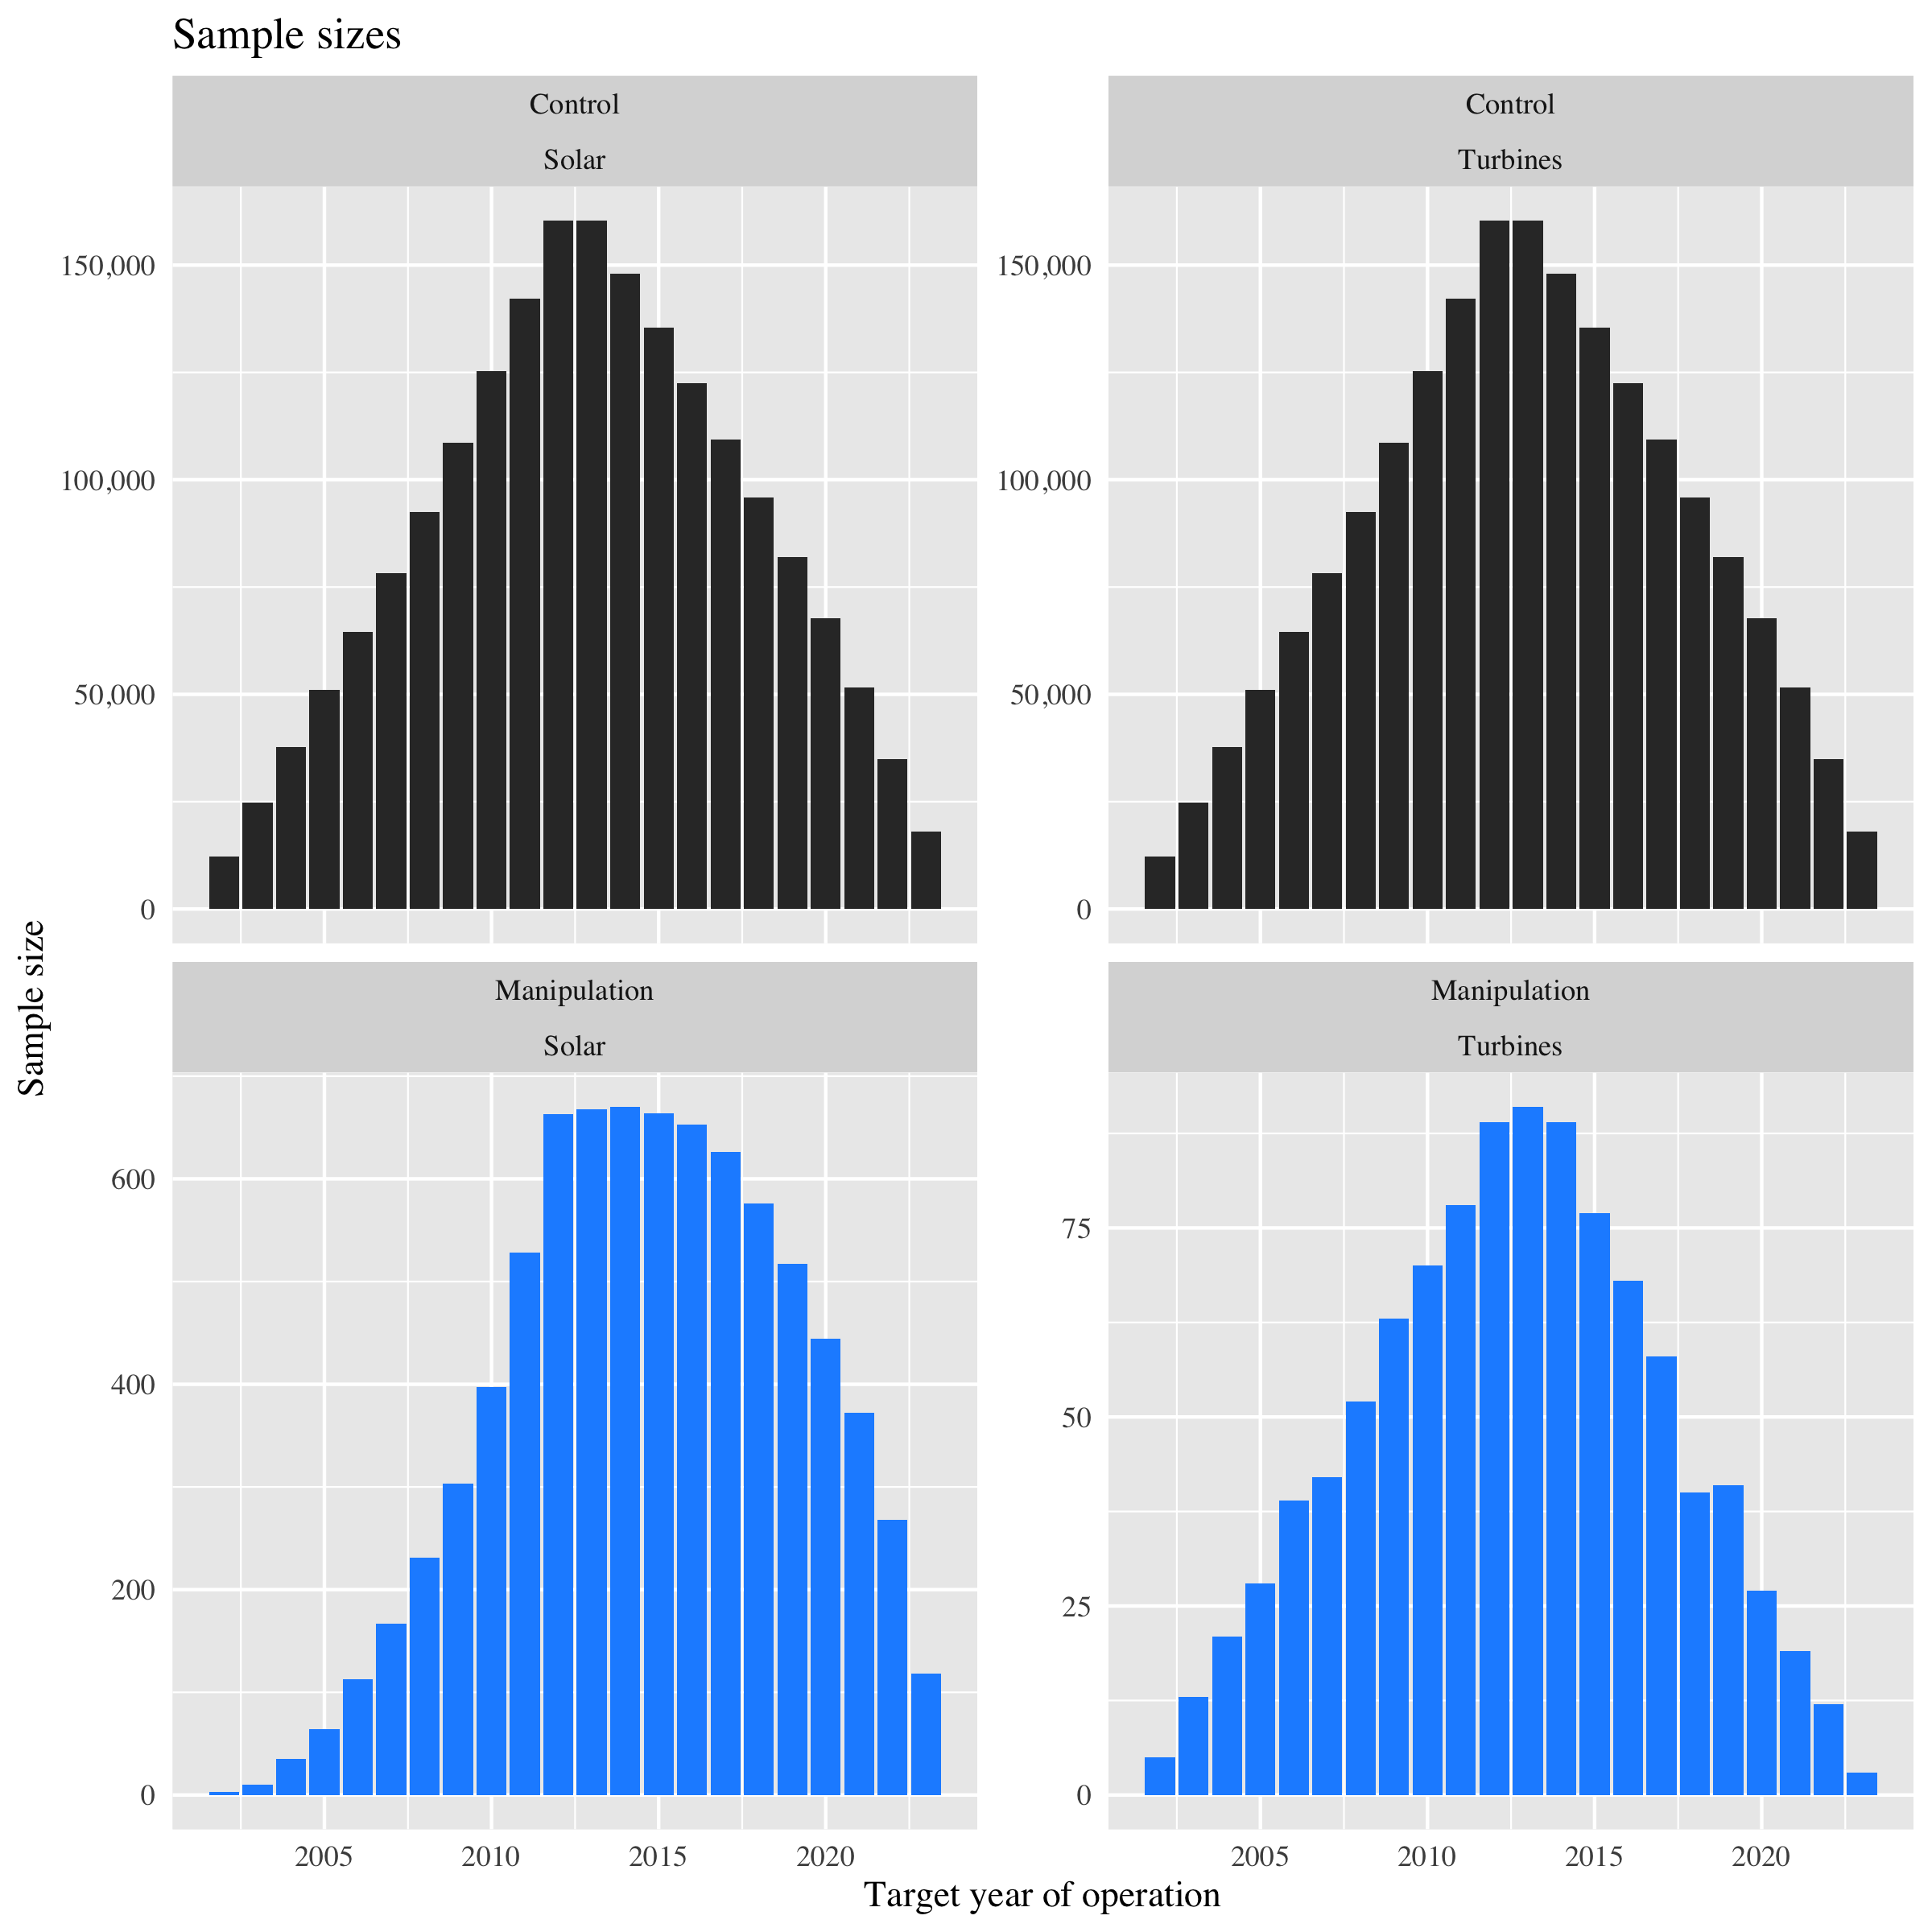
\includegraphics[width=0.9\linewidth]
{study1_sample_size.png} 
\caption{The manipulation groups in the DiD study were extremely small}
\label{study1samplesize}
\end{figure}

\end{document}
